Aunque resulta conveniente usar la diferenciación automática para obtener los
gradientes de una computación, por desgracia hay situaciones donde no es
apropiado su uso. En particular, la diferenciación automática no es aplicable
de manera eficiente a sistemas de ecuaciones lineales, no lineales, ecuaciones
diferenciales ordinarias (ODEs) o ecuaciones diferenciales algebraicas (DAEs),
ni a problemas de optimización.

El motivo principal es que la solución de estos sistemas implica un proceso
iterativo. Esto requeriría almacenar en memoria una gran cantidad de estados
intermedios para realizar la propagación hacia atrás (backward pass) en la
diferenciación automática, lo que resulta computacionalmente costoso y poco
eficiente en términos de memoria.

Por ejemplo, resolver un sistema de ecuaciones lineales típicamente emplea un
método de Krylov como el de gradiente conjugado, que iterativamente modifica
los valores para la solución hasta cumplir con un margen de tolerancia
prestablecido. Para sistemas de ecuaciones no lineales se emplea
Newton-Raphson, y este resuelve una secuencia de sistemas lineales. Sistemas
con ecuaciones diferenciales se discretizan como una secuencia de sistemas
lineales o no lineales para cada paso temporal. Son operaciones claramente
iterativas, que además manejan una gran cantidad de datos (tamaño de las
matrices), y por esto es que almacenar la información de la evaluación original
para su uso con DA en modo reverso se hace inviable.

En su lugar, es más eficiente obtener estas derivadas mediante métodos
semi-analíticos, conocidos como derivadas adjuntas. Estos métodos permiten
calcular los gradientes necesarios sin almacenar todos los estados intermedios,
reduciendo significativamente el uso de memoria y mejorando el rendimiento
computacional, ya que resolver el sistema adjunto para calcular las derivadas
es frecuentemente más simple que el problema directo de solución del sistema.

Adicionalmente, las derivadas adquiridas por DA a través de un problema
iterativo resultan ser menos precisas \cite{scieur2022curse}.

Las técnicas de derivadas adjuntas aprovechan la estructura específica de los
problemas mencionados, consiguiendo los gradientes de manera más directa y
eficiente que la diferenciación automática en estos casos particulares.

Describimos a continuación cómo obtener estas derivadas adjuntas para
diferentes sistemas de ecuaciones que resultan de modelizar sistemas físicos o
de la discretización de ecuaciones en derivadas parciales.

\subsection{Sistemas lineales y no lineales}

Expresamos el sistema de ecuaciones lineales o no lineales en forma residual
(llevando todos los términos a un mismo miembro), y consideramos una función de
agregación $F$ que acepta las variables de estado $y$ junto a las variables de
diseño $x$ como entradas, para producir la salida $f$.

\begin{align}
	r & = R(x, y) = 0 \\
	f & = F(x, y)
\end{align}

En última instancia queremos averiguar los gradientes de las salidas
respecto de las variables de diseño:

\begin{equation} \label{eq:df_dx_adjoint_theory}
	\frac{df}{dx} = \frac{\partial F}{\partial x} + \frac{\partial F}{\partial y} \frac{dy}{dx}
\end{equation}

Para las derivadas parciales de $F$ respecto de $x$ e $y$, podemos aplicar
diferenciación automática a la función $F$, pero con la derivada total
$\frac{dy}{dx}$ necesitamos considerar $R$.

Asumiendo que nos encontramos en un punto donde se satisfacen las ecuaciones
residuales:

\begin{equation}
	\frac{dr}{dx} = \frac{\partial R}{\partial x} + \frac{\partial R}{\partial y} \frac{dy}{dx} = 0
\end{equation}

Podemos hallar $\frac{dy}{dx}$ solucionando el sistema:

\begin{equation} \label{eq:dy_dx_adjoint_theory}
	\frac{\partial R}{\partial y} \frac{dy}{dx} = - \frac{\partial R}{\partial x}
\end{equation}

e incorporando en \eqref{eq:df_dx_adjoint_theory}:

% \frac{df}{dx} = \frac{\partial F}{\partial x} - \underbrace{ \frac{\partial F}{\partial y} \left[\frac{\partial R}{\partial y}\right]^{-1} }_{\psi} \frac{\partial R}{\partial x}
\begin{equation} \label{eq:df_dx_adjoint_two_ways}
	\frac{df}{dx} = \frac{\partial F}{\partial x} - \lefteqn{\overbrace{ \phantom{ \frac{\partial F}{\partial y} \left[\frac{\partial R}{\partial y}\right]^{-1} } }^{\psi} } \frac{\partial F}{\partial y}
	\underbrace{ \left[\frac{\partial R}{\partial y}\right]^{-1} \frac{\partial R}{\partial x} }_{-\frac{dy}{dx}}
\end{equation}

Vemos que es posible encontrar el último término de dos formas distintas.

Una sería multiplicar primero los dos últimos factores de
\eqref{eq:df_dx_adjoint_two_ways}, que es equivalente a lograr $\frac{dy}{dx}$
por \eqref{eq:dy_dx_adjoint_theory}. Ya que $\frac{dy}{dx}$ tiene $n_y$ filas
por $n_x$ columnas, conseguir esta requiere determinar $n_x$ sistemas lineales,
uno por cada columna (entrada).

Este es el método directo. Es la estrategia favorable a seguir cuando el número
de variables de diseño es mayor al número de variables de salida $n_f$.

La alternativa es despejar el producto de los dos primeros factores, aquí llamado
$\psi$, de donde sacamos la relación:

\begin{equation} \label{eq:psi_adjoint_theory}
	\left[ \frac{\partial R}{\partial y} \right]^T \psi = - \left[  \frac{\partial F}{\partial y} \right]^T
\end{equation}

donde $\psi$ es la matriz incógnita, con $n_y$ filas y $n_f$ columnas. El coste
es por tanto el de determinar $n_f$ sistemas lineales, y por eso es atractiva
esta vía cuando el número de salidas es reducido. Conocido como el método
adjunto.

En la figura \ref{fig:direct_adjoint_operations} se visualizan los tamaños de
las matrices empleadas.

\begin{figure}[h]
	\centering
	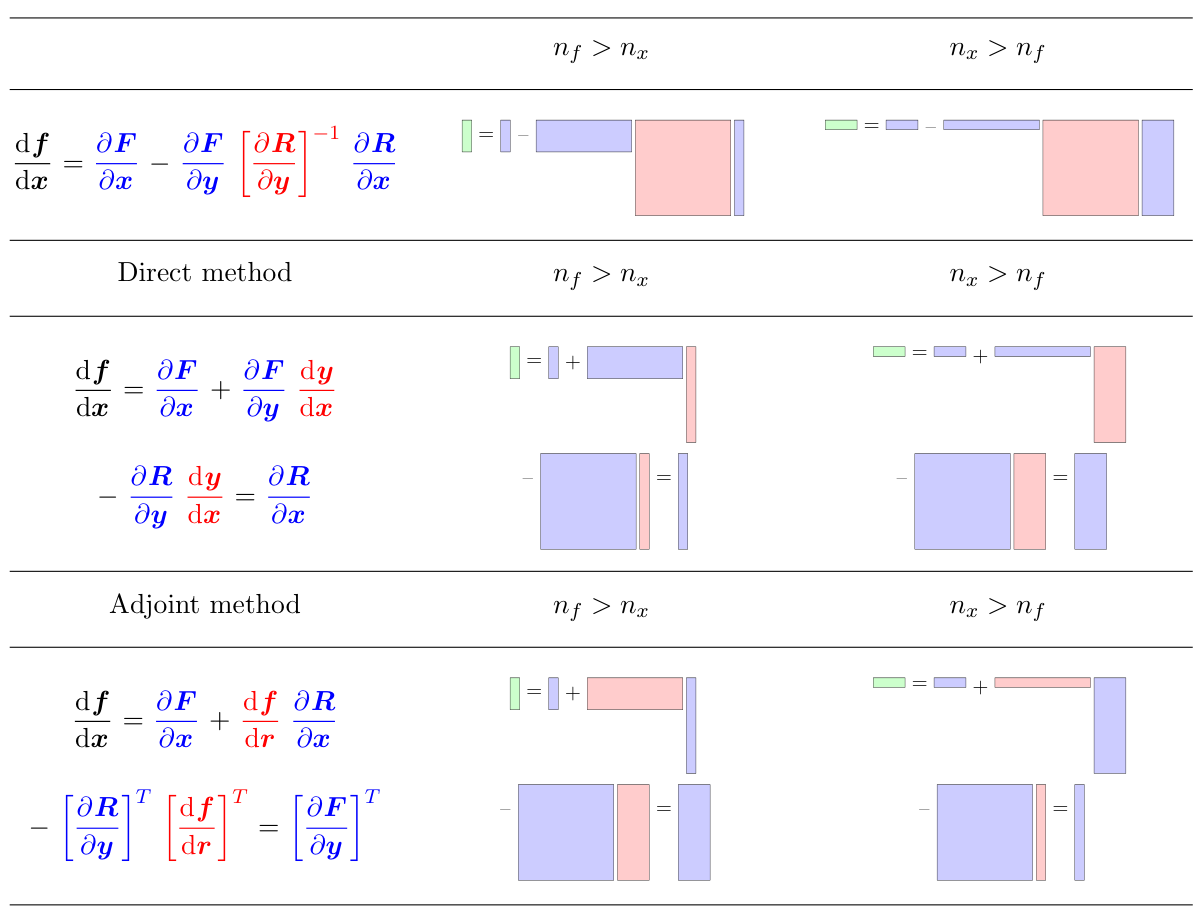
\includegraphics[width=1\textwidth]{./capitulos/metodologia/images/direct_adjoint_operations.png}
	\caption{Métodos directo y adjunto para calcular derivadas semi-analíticas.
		En azul se muestran las matrices de derivadas parciales, sencillas de obtener
		por DA, y en rojo las matrices de derivadas totales que requieren de la
		resolución de sistemas lineales. Se asume que el número de variables de
		estado $n_y$ es mucho mayor que el número de variables de entrada $n_x$ o de
		salida $n_f$ (Adaptado de Martins y Ning \cite{mdobook}, p. 257).}
	\label{fig:direct_adjoint_operations}
\end{figure}


\subsection{ODE's y DAE's}

Al igual que con sistemas de ecuaciones algebraicas, con ecuaciones
diferenciales también consideramos una función de agregación que tomará como
entradas las variables de diseño $x$ y los estados $y$ del sistema ODE
(Ordinary Differential Equation).

\begin{align}
	f             & = F(y(x), x) = \int_{t_0}^{t_N} g(y(x), x) dt \\
	\frac{dy}{dt} & = j(y(x), x, t)  \label{eq:ode_adjoint}       \\
	y(t_0)        & = y_0  \label{eq:ode_adjoint_iv}
\end{align}


Y de nuevo deseamos las derivadas de las salidas respecto de las entradas.


\begin{align}
	\frac{df}{dx} & = \int_{t_0}^{t_N} \frac{d}{dx} g(y;x) dt \nonumber                                                \\
	              & = \int_{t_0}^{t_N} \frac{\partial g}{\partial x} + \frac{\partial g}{\partial y} \frac{d y}{dx} dt
\end{align}


\subsubsection{Método directo contínuo}

Para hallar la derivada total de los estados respecto de las entradas,
derivamos la ODE \eqref{eq:ode_adjoint} con su condición inicial \eqref{eq:ode_adjoint_iv}:

\begin{align}
	\frac{d}{dx_i} \frac{dy}{dt} & = \frac{d}{dx_i} j(y(x), x, t)   \\
	\frac{dy}{dx_i} \big|_{t=0}  & =  \frac{dy_0}{dx_i} \big|_{t=0}
\end{align}

y manipulando, queda un nuevo sistema de ecuaciones diferenciales, donde la
variable de estado ahora sería $\frac{dy}{dx_i}$:

\begin{align}
	\frac{d}{dt} \left( \frac{dy}{dx_i} \right) & = \frac{\partial j}{\partial y} \frac{dy}{dx_i} + \frac{\partial j}{\partial x_i} \\
	\frac{dy}{dx_i} \big|_{t=0}                 & = \frac{dy_0}{dx_i} \big|_{t=0}
\end{align}

por tanto tendremos $n_x$ ODE's que resolver. Este es el método directo
contínuo. Contínuo, porque como veremos a continuación, existe otra forma de
alcanzar las derivadas a partir de la versión discretizada de la ODE (e.g. con
euler implícito).


\subsubsection{Método adjunto contínuo}

En caso de tener muchas variables de diseño $x$, el método directo tiene un
alto coste computacional, por lo que acudimos al método adjunto.

Para lograr las derivadas adjuntas, aquí empleamos el método de la lagrangiana
para su derivación.

Como si formuláramos el siguiente problema de optimización:

\begin{align}
	\min \quad           & F(y, x)   \nonumber                                         \\
	\text{sujeto a}\quad & \frac{dy}{dt}  = j(y, t, x)  \label{eq:ode_as_optimization}
\end{align}

la correspondiente lagrangiana sería:

\begin{align}
	\mathcal{L}(y, x, \lambda) & = F(y, x) + \int_0^T \lambda(t)^T(j - \frac{dy}{dt})dt \nonumber                                   \\
	                           & = \int_0^T g(y, x) + \lambda(t)^T (j - \frac{dy}{dt}) dt  \label{eq:continuous_adjoint_lagrangian}
\end{align}

Derivamos la lagrangiana respecto de las variables de diseño y agrupamos por
$\frac{dy}{dx}$:

\begin{align}
	\frac{d \mathcal{L}}{d x} & = \int_0^T \frac{\partial g}{\partial x} + \frac{\partial g}{\partial y} \frac{dy}{dx} + \lambda(t)^T \left(\frac{dj}{dx} + \frac{\partial j}{\partial y} \frac{dy}{dx} - \frac{d}{d t} \frac{dy}{dx} \right) dt   \nonumber                                              \\
	                          & = \int_0^T  \frac{\partial g}{\partial x} + \lambda(t)^T  \frac{\partial j}{\partial x} + \left(  \frac{\partial g}{\partial y} + \lambda(t)^T  \frac{\partial j}{\partial y} - \lambda(t)^T \frac{d}{dt}  \right) \frac{dy}{dx}  \label{eq:dl_dx_ode_continuous_adjoint}
\end{align}

Integramos por partes el término con la derivada total $\frac{d}{dt}$:

\begin{align}
	\int_0^T -\lambda(t)^T \frac{d}{dt} \frac{dy}{dx} dt = \left[ -\lambda(t)^T \frac{dy}{dx} \right]^T_0 + \int_0^T \frac{dy}{dx} \frac{d\lambda(t)}{dt} dt
\end{align}

Y sustituimos de nuevo en \eqref{eq:dl_dx_ode_continuous_adjoint}:

\begin{align}
	\frac{d \mathcal{L}}{d x} = \int_0^T  \frac{\partial g}{\partial x} + \lambda(t)^T  \frac{\partial j}{\partial x} + \left(  \frac{\partial g}{\partial y} + \lambda(t)^T  \frac{\partial j}{\partial y} + \frac{d \lambda}{dt}^T  \right)  \frac{dy}{dx} + \lambda(0) \frac{dy}{dx}(0) - \lambda(T)^T  \frac{dy}{dx}(T)  \label{eq:dl_dx_ode_continuous_adjoint_1}
\end{align}

Ahora nos gustaría elegir unas variables adjuntas $\lambda$, tal que los
factores para $\frac{dy}{dx}$ y $\frac{d}{dt}(T)$ sean cero. Lo que implica
resolver:

\begin{align}
	\frac{\partial g}{\partial y} + \lambda(t)^T  \frac{\partial j}{\partial y} + \frac{d \lambda}{dt}^T & = 0 \\
	\lambda(T)                                                                                           & = 0
\end{align}

reordenado como:

\begin{align}
	\frac{d \lambda}{dt}^T & = -\frac{\partial j}{\partial y}^T \lambda(t) - \frac{\partial g}{\partial y}^T \\
	\lambda(T)             & = 0
\end{align}

muestra que tenemos una ODE, esta vez de valor final, que se determina hacia
atrás en el tiempo. Y se tienen tantos sistemas como variables de salida $n_f$.

Por último, con $\lambda$ entramos en \eqref{eq:dl_dx_ode_continuous_adjoint_1}
para adquirir:

\begin{equation}
	\frac{d \mathcal{L}}{d x} = \int_0^T \frac{\partial g}{\partial x} + \lambda(t)^T \frac{\partial j}{\partial x} dt + \lambda(0)^T \frac{dy}{dx}(0)
\end{equation}

donde

\begin{equation}
	\frac{dF}{d x} = \frac{d \mathcal{L}}{d x}
\end{equation}

porque el término de la integral en la lagrangiana
\eqref{eq:continuous_adjoint_lagrangian} se hace nulo cuando la ODE se
satisface:

\begin{equation}
	j - \frac{dy}{dt} = 0
\end{equation}


\subsubsection{Método adjunto discreto}

Formulamos el problema de optimización como en \ref{eq:ode_as_optimization},
pero esta vez vamos a discretizar el sistema ODE, por ejemplo con euler
implícito, aunque la misma idea es aplicable para otros métodos explícitos, o
adaptativos.

Las variables de estado se toman como otras variables de diseño a minimizar, y
además hemos añadido variables de control $u$, que en un problema de control
óptimo también son variables de diseño, pero tienen la peculiaridad de que solo
aplican para un paso temporal. Como tenemos un vector de estas a cada instante
de tiempo, si consideramos una trayectoria míninamente larga, tendremos una
gran cantidad de variables de diseño, por lo que el beneficio por usar un
método adjunto es mayor.

Discretizando:

\begin{equation}
	\frac{dy}{dt} = j(x, y, u, t)
\end{equation}

queda:

\begin{align}
	\frac{y_N - y_{N-1}}{h}     & = j(x, y_N, u_N, t_N) \nonumber             \\
	\frac{y_{N-1} - y_{N-2}}{h} & = j(x, y_{N-1}, u_{N-1}, t_{N-1}) \nonumber \\
	                            & \vdots \nonumber                            \\
	\frac{y_{2} - y_{1}}{h}     & = j(x, y_{2}, u_{2}, t_{2}) \nonumber       \\
	\frac{y_{1} - y_{0}}{h}     & = j(x, y_{1}, u_{1}, t_{1})                 \\
\end{align}


que aplicamos como restricciones de igualdad en el problema de optimización:

\begin{align}
	\min_{\mathbf{x}, \mathbf{y}, \mathbf{u}} \quad & F(x, y, u)                                                                  \\
	\text{sujeto a} \quad                           & y_N - y_{N-1} - h \cdot (j(x, y_N, u_N, t_N)) = 0   \nonumber               \\
	                                                & y_{N-1} - y_{N-2} - h \cdot (j(x, y_{N-1}, u_{N-1}, t_{N-1})) = 0 \nonumber \\
	                                                & \vdots \nonumber                                                            \\
	                                                & y_{2} - y_{1} - h \cdot (j(x, y_{2}, u_{2}, t_{2})) = 0 \nonumber           \\
	                                                & y_{1} - y_{0} - h \cdot (j(x, y_{1}, u_{1}, t_{1})) = 0
\end{align}

Con lagrangiana:


\begin{align}
	\mathcal{L} & = F(x, y, u) \nonumber                                                                              \\
	            & - \sum_n \lambda_n \cdot (y_n - y_{n-1} - h \cdot (j(x, y_n, u_n, t_n)))  \label{eq:ode_lagrangian}
\end{align}

Notando que como las ecuaciones del sistema discretizado se cumplen a cada
paso, las derivadas de la lagrangiana respecto de las variables $x$ y $u$ son
iguales a las derivadas de la función objectivo $F$ respecto de $x$ y $u$:

\begin{align}
	\frac{dF}{dx} = \frac{d\mathcal{L}}{dx} \nonumber \\
	\frac{dF}{du} = \frac{d\mathcal{L}}{du}
\end{align}


Así que desarrollamos las condiciones de primer orden de $\mathcal{L}$:

\begin{align}
	\frac{d\mathcal{L}}{dy_n} & = 0 = \frac{\partial F(x, y, u)}{\partial y_n} - \lambda_n + \lambda_n \cdot h \cdot \frac{j(x, y_n, u_n, t_n)}{\partial y_n} + \lambda_{n+1} \label{eq:dl_dy_n_ode} \\
	\frac{d\mathcal{L}}{du_n} & = 0 = \frac{\partial F(x, y, u)}{\partial u_n} + \lambda_n \cdot h \cdot \frac{j(x, y_n, u_n, t_n)}{\partial u_n} \label{eq:dl_du_n_ode}                             \\
	\frac{d\mathcal{L}}{dx}   & = 0 = \frac{\partial F(x, y, u)}{\partial x} + \sum_n \lambda_n \cdot h \cdot \frac{j(x, y_n, u_n, t_n)}{\partial x}  \label{eq:dl_dx_ode}
\end{align}

donde partimos del punto final para sacar primero $\lambda_N$:

\begin{align}
	\frac{d\mathcal{L}}{dy_N} = 0 = \frac{\partial F(x, y, u)}{\partial y_N} - \lambda_N + \lambda_N \cdot h \cdot \frac{j(x, y_N, u_N, t_N)}{\partial y_N} \nonumber \\
	\left(I - h \cdot \frac{j(x, y_N, u_N, t_N)}{\partial y_N} \right) \lambda_N = \frac{\partial F(x, y, u)}{\partial y_N}
\end{align}

con el que averiguamos $\frac{d\mathcal{L}}{du_N}$, y avanzamos hacia $t_0$ como:

\begin{align}
	\frac{d\mathcal{L}}{dy_n}                                                    = 0 = \frac{\partial F(x, y, u)}{\partial y_n} - \lambda_n + \lambda_n \cdot h \cdot \frac{j(x, y_n, u_n, t_n)}{\partial y_n} + \lambda_{n+1} \\
	\left(I - h \cdot \frac{j(x, y_n, u_n, t_n)}{\partial y_n} \right) \lambda_n = \frac{\partial F(x, y, u)}{\partial y_n} + \lambda_{n+1}
\end{align}

finalmente, con todas las variables adjuntas $\lambda$, adquirimos también las derivadas
respecto de $x$ con \eqref{eq:dl_dx_ode}


En otras formulaciones de este mismo método \cite{zhang2022petsc}, se tratan a
las variables de diseño $x$ como parámetros que a pesar de no variar con el
tiempo, tienen una dinámica relacionada:

\begin{equation}
	\frac{dx}{dt} = 0
\end{equation}

y en el problema de optimización se discretizan igualmente:

\begin{align}
	\min_{\mathbf{x}, \mathbf{y}, \mathbf{u}} \quad & F(x, y, u) \nonumber                                                          \\
	\text{sujeto a} \quad                           & y_n - y_{n-1} - h \cdot (j(x, y_n, u_n, t_n)) = 0  \quad \forall n  \nonumber \\
	                                                & x_n - x_{n-1} = 0 \quad \forall n
\end{align}

se conoce también como el sistema aumentado, y la lagrangiana entonces es:

\begin{align}
	\mathcal{L} & = F(x, y, u) \nonumber                                                             \\
	            & - \sum_n \lambda_n \cdot (y_n - y_{n-1} - h \cdot (j(x, y_n, u_n, t_n))) \nonumber \\
	            & - \sum_n \mu_n \cdot (x_n - x_{n-1}) \label{eq:ode_augmented_lagrangian}
\end{align}

aparece una variable adjunta adicional $\mu$. Y haciendo nuevamente las
condiciones de primer orden:

\begin{align}
	\frac{d\mathcal{L}}{dy_n} & = 0 = \frac{\partial F(x, y, u)}{\partial y_n} - \lambda_n + \lambda_n \cdot h \cdot \frac{j(x_n, y_n, u_n, t_n)}{\partial y_n} + \lambda_{n+1} \\
	\frac{d\mathcal{L}}{du_n} & = 0 = \frac{\partial F(x, y, u)}{\partial u_n} + \lambda_n \cdot h \cdot \frac{j(x_n, y_n, u_n, t_n)}{\partial u_n}                             \\
	\frac{d\mathcal{L}}{dx_n} & = 0 = \frac{\partial F(x, y, u)}{\partial x_n} + \lambda_n \cdot h \cdot \frac{j(x_n, y_n, u_n, t_n)}{\partial x_n} - \mu_n + \mu_{n+1}
\end{align}

iniciamos en $t_N$ y a cada paso calculamos $\lambda_n$ y $\mu_n$, y guardamos
la derivada de la función objetivo respecto de las variables de control en ese
paso $\frac{d\mathcal{L}}{du_n}$:

\begin{align}
	\left(I - h \cdot \frac{j(x, y_n, u_n, t_n)}{\partial y_n} \right) \lambda_n & = \frac{\partial F(x, y, u)}{\partial y_n} + \lambda_{n+1}                                                                  \\
	\frac{d\mathcal{L}}{du_n}                                                    & = \frac{\partial F(x, y, u)}{\partial u_n} + \lambda_n \cdot h \cdot \frac{j(x_n, y_n, u_n, t_n)}{\partial u_n}             \\
	\mu_n                                                                        & = \frac{\partial F(x, y, u)}{\partial x_n} + \lambda_n \cdot h \cdot \frac{j(x_n, y_n, u_n, t_n)}{\partial x_n} + \mu_{n+1}
\end{align}

la diferencia es que ahora no necesitamos almacenar las variables adjuntas para
obtener $\frac{d\mathcal{L}}{dx}$ al final del proceso como hacíamos en
\eqref{eq:dl_dx_ode}. Aquí $\frac{dF}{dx}$ es simplemente
$\frac{d\mathcal{L}}{dx_0}$.

Supone un ahorro porque no requerimos los vectores $\lambda$ y $\mu$ en
memoria, solo $\lambda_{n+1}$ y $\mu_{n+1}$ a cada instante $t_n$.


\subsubsection{Diferencias entre el método contínuo y discreto}

Tratando únicamente el modo adjunto, podemos observar ciertas diferencias y
características de los métodos contínuos y discretos.

Como vimos con el método contínuo adjunto, se alcanza un nuevo sistema ODE para
las variables adjuntas $\lambda$, y esta se resuelve hacia atrás en el tiempo,
con una condición final $\lambda(T)$. De esta forma, el método contínuo también
se conoce como "diferenciación y discretización", porque primero diferenciamos
la lagrangiana para formular la ODE de valor final, y después discretizamos el
problema adjunto con algún esquema numérico.

Podemos elegir un esquema de discretización independiente del usado para
determinar el problema directo de la ODE original. Pero esta flexibilidad a
cambio involucra que en la marcha del algoritmo hacia $t = 0$, los puntos ($t$,
$y$) por los que se pase no serán idénticos a los que se visitaron en la
evaluación directa (figura \ref{fig:ode_adjoint_checkpointing_sundials}).
Incluso si usamos el mismo esquema, de ser este adaptativo, es improbable que
los puntos coincidan.

\begin{figure}[h]
	\centering
	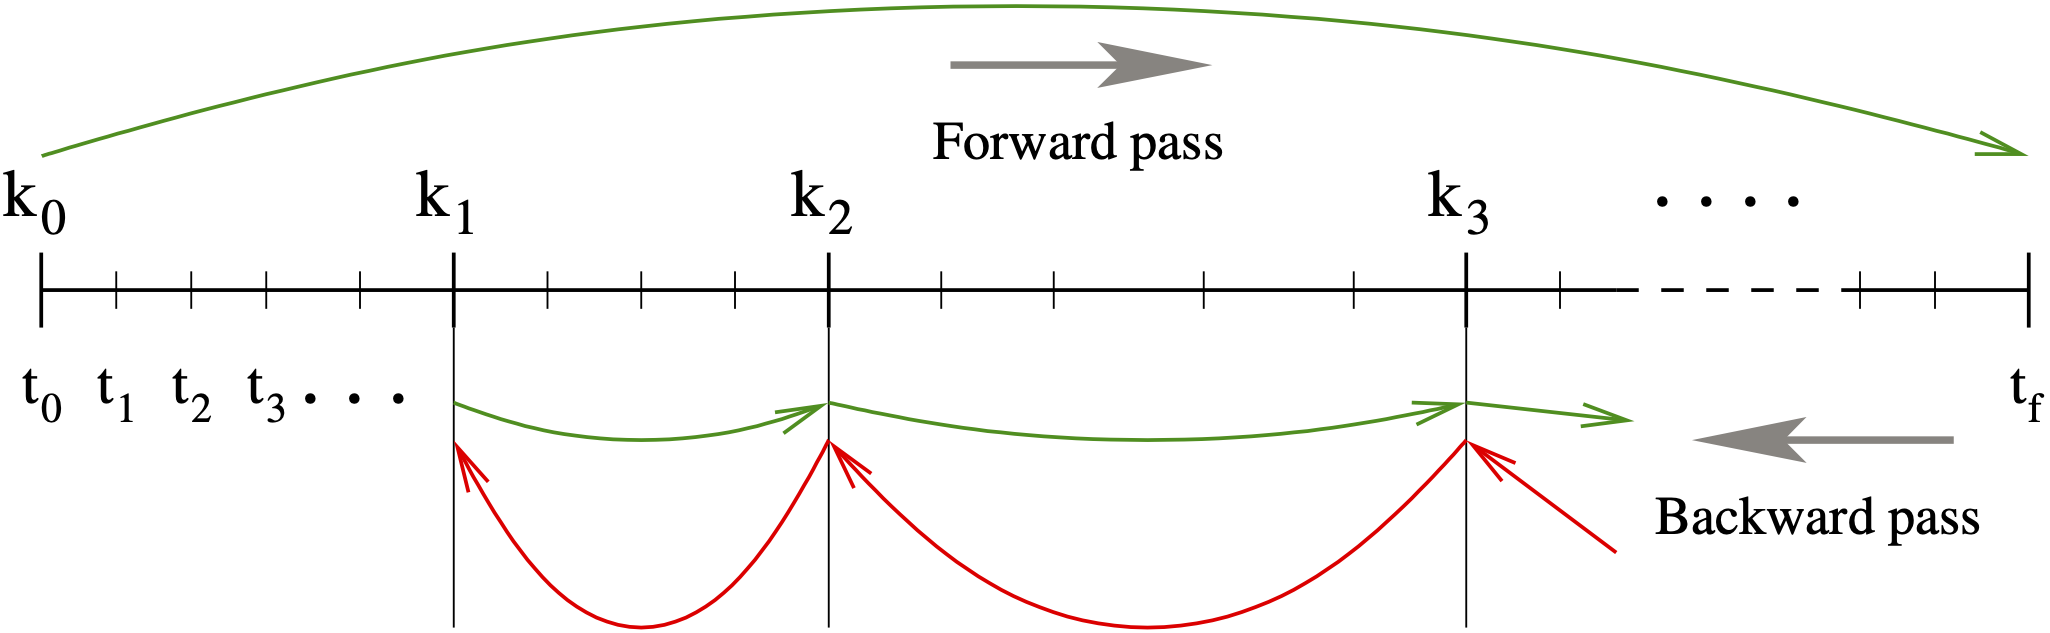
\includegraphics[width=1\textwidth]{./capitulos/metodologia/images/ode_adjoint_checkpointing_sundials.png}
	\caption{Checkpointing realizado por el paquete sundials para obtener las
		derivadas adjoint contínuas a través de un sistema ODE. Fuente:
		\url{https://sundials.readthedocs.io/en/v6.6.0/idas/Mathematics_link.html}}
	\label{fig:ode_adjoint_checkpointing_sundials}
\end{figure}

Pero en la solución de la ODE adjunta para determina $\lambda$, necesitamos de
los valores $t$ y $y$, así que la medida tomada en estos casos es interpolar
entre puntos vecinos, lo que resta precisión numérica y añade coste
computacional.

Por contra, en el método discreto, primero discretizamos el sistema de
ecuaciones diferenciales con algún esquema, y después diferenciamos la
lagrangiana para averiguar las derivadas.

La formulación es dependiente del esquema empleado en el problema directo, pero
a cambio no es preciso interpolar puntos en la pasada hacia atrás, y por tanto
los resultados son más precisos.

\subsubsection{Método adjunto discreto para DAE's}

Ecuaciones diferenciales algebraicas (en inglés DAE: Differential Algebraic
Equation), están compuestas de ecuaciones diferenciales y ecuaciones
algebracias. Su resolución no es idéntica a la de las ODE's, teniendo aspectos
únicos influenciados por cuánto se asemejan a ellas.

Esta semejanza se ilustra con los índices de una DAE.

Existen varios tipos de índices (e.g. índice de Kronecker, índice de perturbación),
pero el más comúnmente empleado es el índice de diferenciación, que es igual
al número máximo de veces que uno debe de diferenciar una ecuación del sistema
para convertir el sistema DAE en uno ODE.

En un caso de muestra con variables de estado $x$ e $y$:

\begin{align} x''(t) + y(t) & = \cos(t) \\
              x             & = cos(t)
\end{align}

para obtener la derivada de $y$ respecto de $t$, debemos de diferenciar la
primera ecuación 1 vez.

\begin{align}
	x'''(t) + y'(t) & = -\sin(t) \\
	x(t)            & = \cos(t)
\end{align}

pero entonces necesitamos una expresión para $x'''$, que conseguimos
diferenciando 3 veces la segunda relación.

\begin{align}
	x'''(t) + y'(t) & = -\sin(t) \\
	x'''(t)         & = -\sin(t)
\end{align}

como fue preciso diferenciar 3 veces una de las ecuaciones, entonces el índice
diferencial de la DAE original es 3.

En general, cuanto mayor es el índice diferencial, mayores problemas uno puede
esperar en la solución numérica.

Paquetes de software como simulink o modelica que modelizan sistemas de
ingeniería formando sistemas de ecuaciones DAE, usan solvers como DASSL
\cite{petzold1982description} o IDA \cite{hindmarsh2005sundials} que
típicamente tratan de reducir el orden utilizando un algoritmo como el de
Pantelides \cite{pantelides1988consistent}.

Y entonces con un sistema DAE de primer orden diferencial, se suele emplear
para su solución un esquema implícito como los empleados con ODE's (e.g.
backward euler).

Pero el desarrollo para adquirir los gradientes adjuntos a través de una DAE
con el método discreto es muy similar al ya explicado para ODE's.

Si tuviéramos un sistema como el siguiente:

\begin{align}
	 & \frac{dy_0}{dt} + p_0 y_0 - p_1 y_1 + p_1 y_1 y_0 + p_1 y_1^2 = 0 \\
	 & \frac{dy_1}{dt} - p_1 y_0^2 + y_1 = 0                             \\
	 & y_2 - 1 + y_0 + y_1 = 0
\end{align}

entonces discretizaríamos de la misma forma las ecuaciones, para luego obtener
la lagrangiana, y con las condiciones de primer orden de esta, resolver las
variables adjuntas desde $t_N$ hasta $t_0$ hacia atrás.

\begin{align}
	\min_{\mathbf{p}, \mathbf{y}} \quad & F(p, y)                                                                                                                                      \\
	\text{sujeto a} \quad               & y_{0_n} - y_{0_{n-1}} + h  p_{0_n}  y_{0_n} - h  p_{1_n}  y_{1_n} + h  p_{1_n}  y_{1_n}  y_{0_n} + h  p_{1_n}  y_{1_n}^2 = 0 \quad \forall n \\
	                                    & y_{1_n} - y_{1_{n-1}} - h  p_{0_n}  y_{0_n}^2 + h  y_{1_n} = 0 \quad \forall n                                                               \\
	                                    & y_{2_n} - 1 + y_{0_n} + y_{1_n} = 0 \quad \forall n
\end{align}


\begin{align}
	\mathcal{L} & = F(p, y) \nonumber                                                                                                                                                                        \\
	            & - \sum_n \lambda_{0_n} \cdot (y_n - y_{n-1} - h \cdot (y_{0_n} - y_{0_{n-1}} + h  p_{0_n}  y_{0_n} - h  p_{1_n}  y_{1_n} + h  p_{1_n}  y_{1_n}  y_{0_n} + h  p_{1_n}  y_{1_n}^2) \nonumber \\
	            & - \sum_n \lambda_{1_n} \cdot (y_n - y_{n-1} - h \cdot (y_{1_n} - y_{1_{n-1}} - h  p_{0_n}  y_{0_n}^2 + h  y_{1_n})) \nonumber                                                              \\
	            & - \sum_n \lambda_{2_n} \cdot (y_n - y_{n-1} - h \cdot (y_{2_n} - 1 + y_{0_n} + y_{1_n}))
\end{align}

Con la diferencia que en la lagrangiana anterior \eqref{eq:ode_lagrangian}
tratábamos con un vector de variables adjuntas $\lambda$, y aquí aparecen
individualmente, para cada ecuación del sistema.
